\documentclass[12pt,a4paper]{article} 

\title{NeuroField User Manual}
\author{Felix Fung \and Romesh Abeysuriya}
\date{\today}

\usepackage{listings}
\usepackage{hyperref}
\usepackage{graphicx}
\usepackage[top=2cm,bottom=2cm,left=1.3cm,right=1.3cm]{geometry}
\usepackage{multirow}
\usepackage{amsmath}

\usepackage{tocloft}
\setlength\cftparskip{4pt}
\setlength{\cftbeforesecskip}{4pt}

\pagestyle{plain}
\parindent=0.0cm
\parskip=0.5cm

\footskip=1.3cm

\lstset{
basicstyle=\small\small\ttfamily,
frame=single,	        % adds a frame around the code
breaklines=true,		% sets automatic line breaking
breakatwhitespace=tru,	% sets if automatic breaks should only happen at whitespace
}
\newcommand{\code}[1]{ 
\begin{lstlisting}
#1
\end{lstlisting}
}
\newcommand{\type}[1]{ {\small\small\tt #1} }

\newcommand{\NF}[0]{ \type{NeuroField}}

\graphicspath{{Figure/}}

\begin{document}

\maketitle

\NF is a \type{C++} program (accompanied with helper scripts) that solves the neural field model of Robinson et al., where each of the simultaneous equations are handled by an object:
\begin{align*}
	P &= \nu_{ab}\phi_{ab}, & \mathtt{Couple}\\
	D_{ab}V_{ab} &= P, & \mathtt{Dendrite}\\
	Q_a &= S_a \big[\sum_b V_{ab} \big], & \mathtt{QResponse}\\
	\mathcal{D}_{ab}\phi_{ab} &= Q_b.&  \mathtt{Propag}
\end{align*}

\NF generalizes the neural field theory by allowing users to:
\begin{enumerate}
	\item Specify an arbitrary population model: an arbitrary number of populations and connections them may be specified;
	\item Specify the parameters for any objects, including populations, dendritic responses, firing responses, propagators, synapses, and stimulus pattern;
	\item Choose alternative wave propagation types, i.e. choose different forms of \(\mathcal{D}_{ab}\);
	\item Uses plastic synapses, i.e. \(\nu_{ab}=\nu_{ab}(\mathbf{r},t)\).
	\item Use different firing responses, i.e. change \(S_a\).
\end{enumerate}

This users guide covers the obtaining and setting up (Sec.~\ref{sec:obtain}), configuring (Sec.~\ref{sec:config}) and launching of \NF (Sec.~\ref{sec:launch}).

Within this documentation, specific terminology as appeared in the computer is in \type{typewriter font}. Commands are denoted as
\begin{lstlisting}
Command to put in computer
\end{lstlisting}

\pagebreak
\tableofcontents

\section{Obtaining and setting up NeuroField}
\label{sec:obtain}

\subsection{Obtaining NeuroField}

The code for \NF is managed by version control system \type{subversion}, which provides a single place to obtain the latest copy of the code, as well as storing the entire history of the program. To access the repository, contact Romesh Abeysuriya (\url{r.abeysuriya@physics.usyd.edu.au}) or Sue Yang (\url{xue.yang@sydney.edu.au}).

To set up the latest version of \NF in the current directory within the School of Physics, execute
\begin{lstlisting}
svn co http://silliac.physics.usyd.edu.au:18080/svn/neurofield/trunk neurofield --username=<your SVN username>
\end{lstlisting}

To obtain a copy of \NF from a computer which is not connected to the School of Physics network (e.g. personal laptops at home), you will require a version of \type{SVN} higher than 1.6. However, you may need to have your IP address/network domain registered for remote access. If you are unable to access the repository remotely, please contact Sebastian Juraszek to request this (ideally by logging a helpdesk request at \url{http://physics.usyd.edu.au/itsupport} - only available within the School of Physics). 

\subsection{Directory layout}

The canonical directory is \type{neurofield/trunk}. Within this directory, the user can find:

\begin{tabular}{l p{14.4cm}}
\type{*.h, *.cpp}& C++ source code.\\
\type{Configs/}& Stores configuration files for \NF.\\
\type{Documentation/}& Contains documentations \type{Documentation/user.pdf} and \type{Documentation/developer.pdf}. Running \type{make doc} generates these documentations.\\
\type{Helper\_scripts/}& Stores helper scripts, including plotting routines and other post-processing of data procedures.\\
\type{Launch}& A launcher script that handles compilation and launching of \NF, capable of automating parameter sweeps and submitting jobs in \type{yossarian}.\\
\type{Output/}& When using the launcher script to sweep over parameters, the launcher script produces this directory, which stores all output files \type{neurofield.*} in independent subdirectories.\\
\type{Release/}& All compiled files, including the object files and the \NF executable is stored here. This directory will be deleted by \type{make clean}, so user data should not be stored here.\\
\type{Test/}& Directory for unit testing and is irrelevant for users.\\
\type{neurofield.*}& Output files generated by \NF.
\end{tabular}

\section{Launching NeuroField}
\label{sec:launch}

The \type{Launch} script is used to compile and launch the \NF program. Users are encouraged to use this script rather than calling the \NF executable directly. To launch \NF, do:

\begin{enumerate}

\item Edit \type{Makefile}: Identify the platform to run NeuroField, and comment/uncomment the appropriate \type{COMP} directions. Generally, this step is not needed, but users are encouraged to check.

\item To execute with only one set of parameters, edit your configuration file in \type{./Configs}, then run
\begin{lstlisting}
./Launch Configs/config_file
\end{lstlisting}
For example,
\begin{lstlisting}
./Launch Configs/cortex.conf
\end{lstlisting}
The output will be stored in the current directory.\footnote{Tips for \type{vi} users: you can launch \NF in \type{vi} with \type{:!./Launch \% [optional params]} }

\item To ease parameter exploration, the launcher script is capable of doing parameter sweeps. The launcher script supports sweeping over an arbitrary number of objects, parameters and runs. For example, if the user wants to launch \NF 3 times, with parameters varying according to the following table,

\begin{tabular}{l l r r r}
Object(s)&Parameter&1\textsuperscript{st} run&2\textsuperscript{nd} run&3\textsuperscript{rd} run\\
\hline
\type{Propag 1}, \type{Propag 2}&\type{gamma}&10&20&30\\
\type{Couple 1}&\type{nu}&1&2&3
\end{tabular}

simply list the above table entries into the argument list:
\begin{lstlisting}
./Launch Configs/cortex.conf 'Propag 1' 'Propag 2' gamma 10 20 30 'Couple 1' nu 1 2 3
\end{lstlisting}

In terms of syntactic restriction, each row in the table can have an arbitary number of objects, but only one parameter; every row must have the same number of runs.\footnote{Tips: the UNIX \type{seq} program allows shortening parameter value listing from \type{10 20 30 40 50 60} into \type{`seq 10 10 60`}, e.g. \type{Launch Configs/cortex.conf 'Propag 1' gamma `seq 10 10 60`}.}

\item Switches are accepted for choosing options. To turn on the switches, put them in the argument list to the launcher script. The following switches are accepted:
	\begin{description}
	\item[\type{--restart}] run \NF in restart mode.
	\item[\type{-i}] specify an configuration file name.
	\item[\type{-o}] specify an output dump file name.
	%\item[\type{-v}] prints to standard output rather than to a file.
	\item[\type{-h}] prints out a list of these switches.
	\end{description}

\item In case the script is executed on \type{yossarian}, the launcher script tries to find a file called \type{pbs}. If no such file is found, the user would be prompted for a job name, expected computational time and email to generate \type{pbs}. This file is then submitted to the PBS system.

\item To clean up the directory, delete or store your \type{neurofield.*} output files and the \type{Output/} directory and subdirectories. Then run
\begin{lstlisting}
make clean
\end{lstlisting}
to delete \type{./Release/} and the files \LaTeX produced in \type{Documentation/}.

\item This documentation can be generated by running 
\begin{lstlisting}
make doc
\end{lstlisting}
which generates \type{./Documentation/user.pdf} and \type{./Documentation/developer.pdf}. \type{make clean} deletes the files (excluding the \type{.pdf} files) created by \LaTeX.

\end{enumerate}

%\section{Using NeuroField executable without launcher script}
%\label{sec:exe}

%It is possible to use the launcher script in virtually all cases, so that a user may skip this section. A notable exception is to restart a completed simulation with a \type{neurofield.dump} file. If a user wishes to use the \type{./Release/NeuroField} executable without the launcher script, then compile it by running
%\begin{lstlisting}
%make
%\end{lstlisting}
%The \NF executable and object files are produced in \type{./Release/}.

%The \type{./Release/NeuroField} executable runs in one of two modes, initial run mode and restart mode.

%(1) In inital run mode \NF takes input from an \type{neurofield.conf} file initializes the simulation and then takes specified number of integration steps writing out a \type{neurofield.output} file and a \type{neurofield.dump} file for restarting.  The input filename can be changed on the command line by using the switch \type{-i newinputfilename}. Similarly the name of the output filename which defaults to \type{neurofield.output} can be changed via the switch \type{-o newoutputfilename}. The dump file which defaults to \type{neurofiled.dump} can be changed via \type{-d newdumpfilename}.

%(2) The code dumps sufficient data about parameter values to restart. In restart mode the simulation will continue where it left off. Restart mode is accessed by running the code with command \type{Neurofield restart} rather than the usual \NF command on the command line. In order to run the code in restart mode it is necessary to take the \type{neurofield.dump} file which was produced from the run which will be restarted to be renamed as the new \type{neurofield.conf} file. The new \type{neurofield.conf} file should also be changed to reflect the new number of timesteps etc.  Note:- A restarting \type{neurofield.conf} file has different content to an initial run \type{neurofield.conf} and can only be used in restart mode.

%A brief description is given by
%\begin{lstlisting}
%./Release/NeuroField --help
%\end{lstlisting}

\section{Writing a configuration file}
\label{sec:config}

\NF allows an arbitrary number of populations and connections between them, with all objects taking arbitrary parameter values. These are all configured via a configuration file. This section documents the specifications of configuration files, where we use \type{Configs/example.conf} as an illustrative example.

To write a configuration file, a user can follow these steps:
\begin{enumerate}
\item Determine your population model by drawing a schematic diagram, thereby constructing a connection matrix. An example is shown in Fig.~\ref{fig:pop}.
\item Look up existing configuration files in \type{Configs/}. By checking the comment located at the top of a configuration file, and also the connection matrix, a user should find the most suitable existing file to construct his own. This is less tedious (and less error prone) than writing a new one from scratch.
\item Specify the global parameters and connectivity matrix (Sec.~\ref{sec:global}).
\item Specify all populations (Sec.~\ref{sec:pop}).
\item Specify all propagators (Sec.~\ref{sec:prop}).
\item Specify all couples (Sec.~\ref{sec:couple}).
\item Specify all output requests (Sec.~\ref{sec:output}).
\end{enumerate}

General rules on the entries within a configuration file:

\begin{enumerate}
	\item The structure of a configuration file is: 1) comment 2) global information 3) object specification 4) output specification.
	\item Object specification involves first specifying the object type. The syntax is the object identifier, followed by its type, then a hyphen:
		\begin{lstlisting}
Object 1: Type -
		\end{lstlisting}
		Then the object parameters are specified, following this pattern:
		\begin{lstlisting}
Object parameter: value
		\end{lstlisting}
	\item Most parameters are essential. Failure to provide these parameters would result in \NF terminating with an error message. A minority of the parameters are optional.
	\item The ordering of the parameters are important. Wrong parameter ordering results in \NF terminating with an error message.
	\item With the exception of keywords, the configuration file is white-space independent, e.g., there can be either no spaces, many spaces, or new lines between the colon of \type{Integration steps: 10000} and 10000, but you cannot have two spaces between \type{Integration} and \type{steps}. For consistency and readability, users are encouraged to follow the existing white space scheme when reasonable.
	\item Tip for \type{vi} users: \type{./helper\_scripts/neurofield.vim} implements syntax highlighting for configuration files in \type{vi}. See comments within for installation instructions.
\end{enumerate}

\begin{figure}[h!]\begin{center}
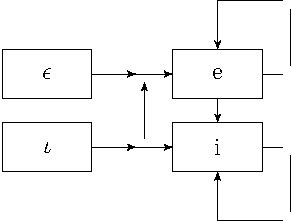
\includegraphics{cortical-model.pdf}
\hspace{3cm}\begin{tabular}{ l l l l l }
	From:& $\epsilon$ & $\iota$ & e & i \\
	To $\epsilon$:& 0 & 0 & 0 & 0 \\
	To $\iota$:& 0 & 0 & 0 & 0 \\
	To e:& 1 & 0 & 2 & 3 \\
	To i:& 0 & 4 & 5 & 6
\end{tabular}
\caption{Left: schematic diagram of a purely cortical population model comprising excitatory and inhibitory populations, as well as two stimulus populations; each arrow indicates a connection between populations, so that each stimulus connects to a cortical population, and each cortical population connects to all cortical populations. Right: connection matrix indicating the connections between populations; zero indicates no connection, and a connection is indicated by a nonzero number, ordered top to bottom, left to right.}
\label{fig:pop}\end{center}\end{figure}

\begin{figure}\begin{center}
	\begin{lstlisting}
Example config file of cortical model with excitatory and inhibitory neurons
Time: 1 Deltat: 1e-4
Nodes: 4 Longside: 2

Connection matrix:
From: 1 2 3 4
To 1: 0 0 0 0
To 2: 0 0 0 0
To 3: 1 0 2 3
To 4: 0 4 5 6

Population 1: Stimulation
 Stimulus: Const - Onset: 0 Mean: 5

Population 2: Stimulation
 Stimulus: Const - Onset: 0 Mean: 5

Population 3: Excitatory neurons
 Q: 8.87145
 Firing: Sigmoid - Theta: 13e-3 Sigma: 3.8e-3 Qmax: 340
  Dendrite 1: V: Steady alpha: 83 beta: 769
  Dendrite 2: V: Steady alpha: 83 beta: 769
  Dendrite 3: V: Steady alpha: 83 beta: 769

Population 4: Inhibitory neurons
 Q: 8.87145
 Firing: Sigmoid - Theta: 13e-3 Sigma: 3.8e-3 Qmax: 340
  Dendrite 4: V: Steady alpha: 83 beta: 769
  Dendrite 5: V: Steady alpha: 83 beta: 769
  Dendrite 6: V: Steady alpha: 83 beta: 769

Propag 1: Map  - phi: Steady Tau: 0
Propag 2: Wave - phi: Steady Tau: 0 Deltax: 3.5e-3 Range: 80e-3 gamma: 116
Propag 3: Map  - phi: Steady Tau: 0
Propag 4: Map  - phi: Steady Tau: 0
Propag 5: Wave - phi: Steady Tau: 0 Deltax: 3.5e-3 Range: 80e-3 gamma: 116
Propag 6: Map  - phi: Steady Tau: 0

Couple 1: Map - nu: .15e-3
Couple 2: Map - nu: 1.5e-3
Couple 3: Map - nu:-1.8e-3
Couple 4: Map - nu: .15e-3
Couple 5: Map - nu: 1.5e-3
Couple 6: Map - nu:-1.8e-3

Output: Node: 1 2 Start: 0 Interval: 1e-4
Population: 4.V
Dendrite: 5
Propag: 1 4.phi
Couple: 3.nu
	\end{lstlisting}
\end{center}
\caption{An example configuration file, which can be found in \type{Configs/example.conf}.}
\end{figure}

\subsection{Global information}
\label{sec:global}
\begin{itemize}

\item
\begin{lstlisting}
Example config file of cortical model with excitatory and inhibitory neurons
\end{lstlisting}
Any text before the entry, \type{Time:}, is disregarded by \NF and serves as comment, which is strongly recommended for all configuration files.
\item
\begin{lstlisting}
Time: 10 Deltat: 1e-4
\end{lstlisting}
\type{Time} is the simulation duration in seconds.

\type{Deltat} is the time increment for each time step.
\item
\begin{lstlisting}
Nodes: 4 Longside: 2
\end{lstlisting}
\type{Nodes} is the number of grid points in the spatial dimension per population of neurons. The code has been explicitly designed to have equal number of neurons per population.

\type{Longside} is an optional parameter, specifying the longside of the rectangular grid. If it is not supplied, it is assumed to be a square.

Both spatial dimensions have periodic boundary conditions, so that populations have the topology of a torus.
\item
\begin{lstlisting}
Connection matrix:
From: 1 2 3 4
To 1: 0 0 0 0
To 2: 0 0 0 0
To 3: 1 0 2 3
To 4: 0 4 5 6
\end{lstlisting}
We specify an arbitrarily sized square connection matrix, where each entry is the connection from the column population to the row population.

Zero indicates no connection.

A nonzero number indicates connection. This number must be indexed from top to bottom, left to right.
\end{itemize}

\subsection{Population data}
\label{sec:pop}
This section contains population information sections. There are two types of neural populations: ordinary populations and stimulus populations:
\begin{description}

\item[Stimulus populations]\ \\

\NF identifies stimulus populations as populations which have no dendrites, i.e., the row for that population contains no nonzero elements.  Each stimulus population information section is as follows.
\begin{itemize}
	\item \begin{lstlisting}
Population 1: Stimulation
	\end{lstlisting}
	The identifier \type{Population 1} is required for cross-checking.

	The descriptor \type{Stimulation} is not parsed by \NF, but it is strongly recommended for human referencing.
	\item
	\begin{lstlisting}
Stimulus: Const - Onset: 0
	\end{lstlisting}
	The identifier \type{Stimulus} is required for cross-checking.

	This is followed by the type of stimulus, to be further elaborated below.

	Optional parameter \type{Onset} specifies the time onset for the stimulus to begin. If unspecified, stimulus starts at time 0.

	Either \type{Cease} or \type{Duration} can be an optional parameter to specify the end time of the stimulus. If unspecified, stimulus ends at 1000 seconds.

	Possible stimulus patterns:

	\textbf{Constant}
	\begin{lstlisting}
Const - Mean: 5
	\end{lstlisting}

	\textbf{Pulse}
	\begin{lstlisting}
Pulse - Amplitude: 1 Width: 2e-2 Frequency: 1 Pulses: 1
	\end{lstlisting}

	\textbf{White noise stimulus}
	\begin{lstlisting}
White - Amplitude: 20 Mean: 1
	\end{lstlisting}

    One issue with white noise is that the power spectrum of white noise depends on both the temporal sampling rate and the grid size. For a thorough discussion of this phenomenon, see \type{noise.pdf} in the \NF documentation. Therefore, if you change the sampling rate, the number of nodes, or \type{Deltax} then the power spectrum will change in amplitude. If you know what amplitude the noise should have in Fourier space e.g. $\phi_n(\omega) = 1 \times 10^{-5}$ then specifying \type{Deltax} in the stimulus population will tell \NF that the amplitude has been specified in Fourier space, and it will be rescaled accordingly. In this representation, the mean of the distribution corresponds to the zero-frequency component of the noise. 
    
	\begin{lstlisting}
White - Amplitude: 0.00001 Mean: 1 Deltax: 0.025
	\end{lstlisting}
	
	Whether \type{Deltax} is specified or not, you can always optionally specify the seed for the random number generator. If you do not specify a seed, an automatically-incremented seed will be used instead, so that multiple stimulus populations will have independent sequences. In general it is not necessary to set the seed manually unless different random numbers are required for otherwise identical runs. 

	\begin{lstlisting}
White - Amplitude: 0.00001 Mean: 1 Ranseed: 10
	\end{lstlisting}
	\begin{lstlisting}
White - Amplitude: 0.00001 Mean: 1 Deltax: 0.025 Ranseed: 10
	\end{lstlisting}

	To superimpose 2 or more stimuli, begin with the keyword \type{Superimpose}, followed by the number of stimuli. Then list all the stimulus patterns and their parameters, with each stimulus pattern preceded by the keyword \type{Stimulus}.
	\begin{lstlisting}
Stimulus: Superimpose: 2
 Stimulus: White - Amplitude: 1 Mean: 1
 Stimulus: Pulse - Onset: 0.5 Width: 2e-2 Frequency 1 Pulses: 1
	\end{lstlisting}

	\end{itemize}
\item[Ordinary populations]\ \\
	Any non-stimulus population is an ordinary population.

	\begin{itemize}
	\item
	\begin{lstlisting}
Population 3: Excitory neurons
	\end{lstlisting}
	The identifier \type{Population 3} is required for cross-checking.
	
	The descriptor \type{Excitatory neurons} is not parsed by \NF, but it is strongly recommended for human referencing.
	\item
	\begin{lstlisting}
Q: 8.87145
	\end{lstlisting}
	The initial firing rate.
	\item
	\begin{lstlisting}
Firing: Sigmoid - Theta: 13e-3 Sigma: 3.8e-3 Qmax: 340
	\end{lstlisting}
	Specify the sigmoidal firing response of the population.

	\type{Sigma} is sometimes known as \(\tilde{\sigma}\). It is already scaled by \(\pi/\sqrt{3}\).

	Alternatively, you can specify a linear firing response by using
	\begin{lstlisting}
Firing: Linear - Gradient: 1 Intercept: 1
	\end{lstlisting}

	\item
	\begin{lstlisting}
Dendrite 1: V: Steady alpha: 83 beta: 769
	\end{lstlisting}
	The identifier \type{Dendrite 1}, where the number 1 is the presynaptic connection index, is required for cross-checking. Users should find that these indices are simply ordered as 1, 2, 3, 4, ...
	
	Optional parameter \type{V} may be used to specify the initial depolarization contribution from presynaptic activity. If unspecified, or set to \type{Steady}, \NF calculates the initial value by \(V_{ab}=\nu_{ab}\phi_{ab}\).

	\type{alpha} and \type{beta} are the parameters for the depolarization response.
	\end{itemize}
\end{description}

\subsection{Propagation data}
\label{sec:prop}
\begin{itemize}
\item
	\begin{lstlisting}
Propag 1:
	\end{lstlisting}
	This identifier is required for cross-checking.
\item A propagator type is required at this point. Choices are \type{Map}, \type{Wave}, and \type{Harmonic}.
\begin{description}
	\item[Map]\ \\
	\begin{lstlisting}
Map - phi: Steady Tau: 0
	\end{lstlisting}
	This propagator is the mapping propagator where spatial spreading is negligible. Its form is given by
	\[\phi_{ab}({\bf r}, t) = Q_b ({\bf r}, t - \tau_{ab}).\]
	Its only one parameter, \type{Tau}, is the the delay term. It is specified below.

	Optional parameter \type{phi} may be used to specify the initial axonal firing rate. If unspecified, or set to \type{Steady}, \NF calculates the initial value by \(\phi_{ab}=Q_{b}\).

	\item[Wave]\ \\
	This propagator is the wave equation propagator governed by the equation
	\[\left[\frac{1}{\gamma_{ab}^2}\frac{d^2}{d t^2}+\frac{2}{\gamma_{ab}}\frac{d} {d t}+1 -r^2_{ab}\nabla^2 \right] \phi_{ab}({\bf r},t) =Q_b({\bf r},t-\tau_{ab}).\]
	Its input is given by
	\begin{lstlisting}
Wave - phi: Steady Tau: 0 Deltax: 3.5e-3 Range: 80e-3 gamma: 116
	\end{lstlisting}

	Optional parameter \type{phi} may be used to specify the initial axonal firing rate. If unspecified, or set to \type{Steady}, \NF calculates the initial value by \(\phi_{ab}=Q_{b}\).

	\type{Deltax} is the length of a node in mm. This must satisfy the Courant condition, \[\Delta t/\Delta x<\sqrt{2}/r_e\gamma_e.\]

	\type{Range} is $r_{ab}$ in the wave equation.
	
	\type{gamma} is the damping coefficient. Alternatively, \type{velocity} may be specified, and \type{gamma} is calculated via \(\gamma_{ab}=\mathrm{v}_{ab}/r_{ab}\).

	In case there is only one node, this degenerates into a \type{Harmonic} propagator.

	\item[Harmonic]
	This is a harmonic oscillator implementation of the damped wave equation, with no spatial variations:
	\[\left[\frac{1}{\gamma_{ab}^2}\frac{d^2}{d t^2}+\frac{2}{\gamma_{ab}}\frac{d} {d t}+1 \right] \phi_{ab}({\bf r},t) =Q_b({\bf r},t-\tau_{ab}).\]

	The input form is given by 
	\begin{lstlisting}
Harmonic - phi: Steady Tau: 0 gamma: 116
	\end{lstlisting}

	\item[Tau]\ \\
	The axonal time delay between populations. If it is spatially homogeneous, then it is a number with units of seconds. If it is spatially inhomogeneous, then input \(n\) numbers, where \(n=\) \type{Nodes}.

\end{description}
\end{itemize}

\subsection{Coupling data}
\label{sec:couple}

\begin{itemize}

	\item
	\begin{lstlisting}
Couple 1:
	\end{lstlisting}
	Identifier for cross-checking.
\item A couple type is required at this point. Choices are \type{Map}, \type{CaDP}, \type{BCM} and \type{Matrix}.

\begin{description}

	\item[Map]\ \\
	Nonplastic synaptic coupling wtih a single constant parameter \type{nu},
	\begin{lstlisting}
Map - nu: 0.0012
	\end{lstlisting}
	\type{nu} is the synaptic coupling parameter. It corresponds to the product of the mean synaptic strength $s_{ab}$ and $N_{ab}$, the mean number of connections from cells of type $b$ to cells of type $a$.

	%\item[Modcouple]\ \\
	%The modulated synaptic coupling implements the Clearwater/Rennie modulation equation. The modulation is given by
	%\[ \nu (t) = \nu_0 \left[ ( 1 - \nu_{scal} ) e^{h(t)/k} + \nu_{scal} \right], \]
	%where $h(t)$ is the time low passed filtered form of the neuromodulators concentration $C(t)$ as given by
	%\[
	%\left\{ \frac{1}{\mu \lambda} \frac{d^2}{dt^2} +
	%\left[ \frac{1}{\nu}+ \frac{1}{\lambda} 
	%\right]
	%\frac{d}{dt} + 1
	%\right\}
	%h(t) = C(t).
	%\]
	%The neuromodulator's concentration is in turn given by a user chosen stimulus form analogous to stimulus populations.

	%The remainder of the input form is specification of the output for $\nu$.  This takes an analogous form to the usual output data lines. The $\nu$ data is output to a file with filename \type{neurofield.synaptout.xx} where xx is an index number of the coupling.

	%An example Modcouple input form is given by
	%\begin{lstlisting}
%ModCouple - Nuzero: 0.0002 Nuscal: 0.02 Mu: .1 Lambda: 1 k: .000001
%Concentration mode: 1  Time to start of Concentration: .01 Amplitude: .0001
%Pulse Duration: .2 Pulse repetition period: 40
%Number of traces: 100  Single/All: All nodes}
	%\end{lstlisting}

	\item[Matrix]\ \\
	Coupling becomes connection matrix, where connection strength does \emph{not} change with time. The format of the nu matrix is the same as the population connection matrix, each row is to the same node, each column is from the same node. When outputting, each specified outputting node output the indexed row.
	\begin{lstlisting}
nu:
  13e-6 0
  0 13e-6
	\end{lstlisting}

	\item[CaDP]\ \\
	Calcium dependent plasticity according to Fung and Robinson.
	\begin{lstlisting}
CaDP - nu: 13e-6 nu_max: 80e-6 Dth: .25e-6 Pth: .45e-6 xyth: 1e-4 x: 2.3e-2 y: 2e-2 B: 30e3 glu_0: 200e-6 gNMDA: 2e-3
	\end{lstlisting}

	\type{Dth} and \type{Pth} are the calcium-plasticity thresholds; \type{xyth}, \type{x} and \type{y} are the plasticity rates; \type{B}, \type{glu\_0} and \type{gNMDA} are NMDA receptor parameters.

	To use \type{CaDP}, glutamate dynamics must be specified for the postsynaptic population. In the end of the relevant population entry, append
	\begin{lstlisting}
Glutamate dynamics - Lambda: 150e-6 tGlu: 30e-3
	\end{lstlisting}
	\type{Lambda} is the glutamate concentration rise per presynaptic spike; \type{tGlu} is the decay timescale for glutamate dynamics.

	\item[BCM]\ \\
	Extends \type{CaDP} with metaplasticity according to Fung and Robinson. it has an additional parameter \type{t\_BCM}, the timescale of metaplasticity.
	\begin{lstlisting}
CaDP - nu: 13e-6 nu_max: 80e-6 Dth: .25e-6 Pth: .45e-6 xyth: 1e-4 x: 2.3e-2 y: 2e-2 B: 30e3 glu_0: 200e-6 gNMDA: 2e-3 t_BCM: 7
	\end{lstlisting}

\end{description}
\end{itemize}

\subsection{Output data}
\label{sec:output}

\NF outputs field quantities (i.e. a neurodynamic quantity which takes a value for each node) with respect to nodes and time. By default, the output file is \type{neurofield.output}, which can be changed by launching the program with the \type{-o} switch.

\begin{itemize}
	\item \begin{lstlisting}
Output:
		\end{lstlisting}
Begin with the \type{Output} declaration.
\item \begin{lstlisting}
Node: 1 2
\end{lstlisting}
Enumerate all nodes to be outputted. If outputting all nodes, use shorthand \type{All}. If no nodes are specified, no nodes will be outputted.
\item \begin{lstlisting}
Start: 0 Interval: 1e-4
\end{lstlisting}
Optional parameters for the time to start output, and optional parameter for time interval between outputs.

If undefined, defaults, to 0 and \type{Deltat}, respectively.
\item \begin{lstlisting}
Population: 4.V
Dendrite: 5
Propag: 1 4.phi
Couple: 3.nu
\end{lstlisting}
Specifying desired objects and fields to output. Enter the appropriate object indices after the labels.

For each entry, a field name may be appended after the index with a \type{.}, so that only that field of the object is outputted. If no field name is specified for that entry, then all fields of that object is outputted.

If a specific field of an object is specified, but that field does not exist, \NF checks and returns an error.

\end{itemize}

\section{Postprocessing}

\NF produces 3 files:

\begin{tabular}{l p{14.4cm}}
\type{neurofield.conf}& When using the launcher script, this file is created to store the running configuration file.\\
%\type{neurofield.dump}& \NF dumps data here when it terminates. This file can be used in restart mode to continue simulation. Creation of this file can be suppressed by a \type{-s} switch.\\
\type{neurofield.output}& The result of the simulation is stored here for postprocessing.\\
\type{neurofield.pbs}& If \NF is run in \type{yossarian}, then this file stores the output of the queueing system.
\end{tabular}

When the launcher script runs with only one set of parameters, all output files are also in the present working directory. However, if the launcher script sweeps over parameters, each parameter set has its own subdirectory inside \type{Output/}, and each set of \type{neurofield.*} files are stored in its subdirectory.

Example content in \type{neurofield.output} is
\begin{lstlisting}
                Time  |          Propag.2.phi
                      |                     0
1.00000000000000e-04  |  8.87145000000000e+00
\end{lstlisting}

Each column is a time series with its name indicated in the first line. The first column is always time, and in this example, the second column is \type{Propag.2.phi}, indicating that it is $\phi_{ee}$ (when checked against connection matrix). The delimiter \type{|} indicates that the two columns are different fields, rather than different nodes of the same field. The node number is indicated in the second line.

It is also worth noting that traces will be written in the order that they are specified. For example, if you write \type{Population: 3 1} then the columns in the output file will be arranged in this order. 

\subsection{Quickplot}

The data in \type{neurofield.output} may be plotted by \type{./Helper\_script/quickplot.pl} or in \type{MatLab} via the matlab scripts within \type{./Helper\_script/}.

To use \type{./Helper\_script\/quickplot.pl}, execute
\begin{lstlisting}
./Helper_script/quickplot.pl [output.file] [field] [node index]
\end{lstlisting}
where an example is
\begin{lstlisting}
./Helper_script/quickplot.pl neurofield.output Propag.2.phi 1
\end{lstlisting}
or a shorthand to plot all fields and nodes is
\begin{lstlisting}
./Helper_script/quickplot.pl all
\end{lstlisting}
All these commands launches \type{gnuplot} plotting sessions.

\subsection{Matlab}
A number of Matlab functions are provided to make it easy to manipulate \NF data from within Matlab. The functions are generally self-documenting with comments at the start of the file.

Essentially, an output file from \NF is read into a \type{nf} struct object in Matlab which simply contains all of the output from \NF in memory for easy access. Here is an example of a \type{nf} object:
\begin{lstlisting}
     fields: {'Propag.1.phi'  'Propag.3.phi'}
      nodes: {[1]  [1]}
       data: {[300000x1 double]  [300000x1 double]}
       time: [300000x1 double]
     deltat: 1.0000e-04
    npoints: 300000
\end{lstlisting}
\begin{itemize}
\item \type{fields} stores a record of which traces from \NF are present in the output file
\item \type{nodes} is a cell with the same size as \type{fields}, and records for each field present, the number of the node in the output. 
\item \type{data} is a matrix storing the actual values of the traces
\item \type{time} is a vector of time values, so that you can plot any of the data traces directly again \type{nf.time}
\item \type{deltat} stores the temporal sampling rate
\item \type{npoints} stores the total number of points in the output. The total duration is \type{nf.deltat*nf.npoints} (or  \type{nf.time(end)})
\end{itemize}

There are two ways to create the \type{nf} object. You can read the output file directly after executing \NF elsewhere

\begin{lstlisting}
nf = nf_read('neurofield.output')
\end{lstlisting}

or you can use the \type{nf\_run} helper script to run the config file using \NF and automatically parse the output

\begin{lstlisting}
nf = nf_run('neurofield.conf')
\end{lstlisting}

Using \type{nf\_run} means you will need to add \NF to your shell search path.

Several helper files are provided to manipulate the \type{nf} object. The two most important helpers are \type{nf\_extract} and \type{nf\_grid}. Often you want to extract a particular field from the \type{nf} object, for example, to examine the output from \type{Propag.3.phi}. To do this directly with the \type{nf} object, you would need to check the \type{fields} variable to find the index of the trace you wanted, and then extract it from the \type{data} field. In the previous example, \type{Propag.3.phi} is the second trace. These expressions are identical:
\begin{lstlisting}
trace = nf.data{2};
trace = nf_extract(nf,'Propag.3.phi')
\end{lstlisting}
\type{nf\_extract} quickly becomes useful when there are many different fields. It is not case sensitive (so \type{propag.3.phi} works as well). You can also specify using additional arguments to extract only a portion of the time series, and also to select a subset of nodes. Finally, you can also provide multiple traces to concatenate them into a single matrix. For example,
\begin{lstlisting}
trace = nf_extract(nf,'propag.1.phi,propag.3.phi');
\end{lstlisting}
will create a 300000$\times$2 matrix with both of the traces. 

Finally, if you run \NF with multiple nodes, it typically solves the system of equations on a square grid. Therefore, if you have output for notes 1-400, this corresponds to a 20$\times$20 grid. \type{nf\_grid} allows you to request a trace from the \type{nf} object and have it reshaped into a square grid. This lets you easily make surface plots of the data, or perform tasks that are spatially dependent. 

One important task is computing the power spectrum as predicted by the linearized analytic equations. This can be achieved using \type{nf\_spatial\_spectrum} which takes in an \type{nf} object and computes the power spectrum integrated over $k$ taking into account volume conduction. 

\end{document}
